\documentclass[a4paper]{article}
\usepackage[a4paper,margin=0mm]{geometry}
\usepackage{fontspec}
\usepackage{unicode-math}
\usepackage{tikz}
\usepackage[table]{xcolor}
\usepackage[absolute]{textpos}
\usepackage{enumitem}
\usepackage{array}
\usepackage{multirow}

\setmainfont{Libertinus Serif}
\setsansfont{Libertinus Sans}
\setmathfont{Libertinus Math}
\newfontfamily\trackedsans{Libertinus Sans}[LetterSpace=8.0]

\definecolor{accent}{HTML}{602785}
\definecolor{badge}{HTML}{B8A0C8}
\definecolor{ink}{HTML}{2A2E30}

\setlength{\TPHorizModule}{1mm}
\setlength{\TPVertModule}{1mm}
\setlength{\parindent}{0pt}
\pagestyle{empty}

\newcommand{\LCOL}{16mm}
\newcommand{\RCOL}{111mm}
\newcommand{\COLW}{83mm}

\newcommand{\topicheader}[2]{%
\begin{textblock*}{194mm}(16mm,10mm)
\begin{tikzpicture}
\node[fill=accent,text=white,font=\sffamily\bfseries\fontsize{13}{13}\selectfont,
      minimum width=9mm,minimum height=9mm,inner sep=0pt] at (4.5mm,-4.5mm) {#1};
\node[font=\sffamily\bfseries\fontsize{15}{16}\selectfont,text=ink,anchor=west] at (12mm,-4.5mm) {#2};
\end{tikzpicture}
\end{textblock*}
\begin{textblock*}{194mm}(16mm,22.5mm)

\begin{tikzpicture}
\fill[accent] (0,0) rectangle (194mm,0.5mm);
\end{tikzpicture}
\end{textblock*}
}

\newcommand{\pagefooter}[1]{%
\begin{textblock*}{194mm}(8mm,286.41mm)
  
\begin{tikzpicture}
    \fill[accent] (0,0) rectangle (194mm,0.6mm);
  \end{tikzpicture}
\end{textblock*}
\begin{textblock*}{63.59mm}(8mm,288.27mm)
  {\sffamily\bfseries\color{accent}\fontsize{13}{16}\selectfont SAT 1200+}
\end{textblock*}
\begin{textblock*}{10mm}(188mm,288.27mm)
  \centering{\sffamily\color{accent}\fontsize{14}{16}\selectfont #1}
\end{textblock*}
}

\newcommand{\colrule}[2]{%
\begin{textblock*}{1mm}(105mm,#1mm)
\begin{tikzpicture}
\draw[black!65,line width=0.5pt] (0,0) -- (0,#2mm);
\end{tikzpicture}
\end{textblock*}
}

\newcommand{\setkicker}[2]{%
{\sffamily\bfseries\fontsize{12}{14}\selectfont #1.}\ {\itshape\fontsize{11}{14}\selectfont\color{black!75} #2}\par\vspace{2mm}%
}

\setlength{\fboxsep}{1.4pt}
\setlength{\fboxrule}{0.5pt}
\newcommand{\pnum}[1]{\fcolorbox{ink}{white}{\sffamily\bfseries\fontsize{8}{8}\selectfont #1}~}

\newcommand{\qrbox}[1]{%
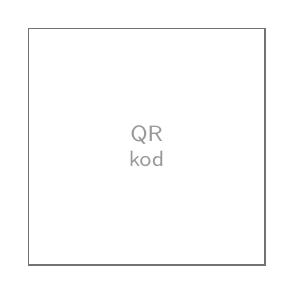
\begin{tikzpicture}
\draw[black!55,line width=0.6pt] (0,0) rectangle (30mm,30mm);
\node[black!40,font=\sffamily\fontsize{8}{9}\selectfont,align=center] at (15mm,15mm) {QR\\kod};
\end{tikzpicture}\\[1.5mm]
{\sffamily\fontsize{9}{11}\selectfont\color{black!70} #1}%
}

\arrayrulecolor{accent}
\setlength{\arrayrulewidth}{0.7pt}
\renewcommand{\arraystretch}{1.35}
\newcommand{\anstitle}[1]{{\sffamily\bfseries\color{accent}\fontsize{11}{13}\selectfont #1}\\[1.3mm]}

\begin{document}

% ================= PAGE 1: Set 1 | Set 2 =================
\topicheader{23}{Pifagor Teoremasi va Koordinatalar}
\pagefooter{123}
\colrule{32}{238}
\mbox{}%

\begin{textblock*}{\COLW}(\LCOL,32mm)
{\fontsize{12}{15}\selectfont
\setkicker{1-to'plam}{Har doim to'g'ri burchak berilgan -- yetishmayotgan tomonni toping.}

\noindent\pnum{1} Katetlar $3$ va $4$. Gipotenuza?\\[26mm]
\noindent\pnum{2} Katetlar $6$ va $8$. Gipotenuza?\\[26mm]
\noindent\pnum{3} Katetlar $5$ va $12$. Gipotenuza?\\[26mm]
\noindent\pnum{4} Gipotenuza $10$, bir katet $6$. Ikkinchi katet?\\[26mm]
\noindent\pnum{5} Gipotenuza $13$, bir katet $5$. Ikkinchi katet?\\[26mm]
\noindent\pnum{6} Gipotenuza $17$, bir katet $8$. Ikkinchi katet?
}
\end{textblock*}

\begin{textblock*}{\COLW}(\RCOL,32mm)
{\fontsize{11}{14}\selectfont
\setkicker{2-to'plam}{Qo'llash mumkinmi? Avval hal qiling, keyin hisoblang.}

\noindent\pnum{1} To'g'ri burchak $9$ va $12$ katetlar orasida. Gipotenuza?\\[14mm]
\noindent\pnum{2} Tomonlari $7$, $8$, $10$. Burchak berilmagan. Pifagor teoremasi shu yerda ishlatilishi mumkinmi?\\[11mm]
\noindent\pnum{3} Tomonlari $8$, $15$, $17$. Teskari tekshiruv: bu to'g'ri burchakli uchburchakmi?\\[11mm]
\noindent\pnum{4} Tomonlari $6$, $8$, $11$. Teskari tekshiruv: bu to'g'ri burchakli uchburchakmi?\\[11mm]
\noindent\pnum{5} To'g'ri burchak $7$ va $24$ katetlar orasida. Gipotenuza?\\[14mm]
\noindent\pnum{6} Teng yonli uchburchak: tomonlari $10$, $10$, asos $12$. Bu to'g'ri burchaklimi?
}
\end{textblock*}

\clearpage

% ================= PAGE 2: Set 3 | Set 4 =================
\topicheader{23}{Pifagor Teoremasi va Koordinatalar}
\pagefooter{124}
\colrule{32}{238}
\mbox{}%

\begin{textblock*}{\COLW}(\LCOL,32mm)
{\fontsize{12}{15}\selectfont
\setkicker{3-to'plam}{Masofa formulasi -- mashq.}

\noindent\pnum{1} $(0,0)$ va $(3,4)$\\[26mm]
\noindent\pnum{2} $(2,3)$ va $(7,15)$\\[26mm]
\noindent\pnum{3} $(-4,1)$ va $(4,7)$\\[26mm]
\noindent\pnum{4} $(1,1)$ va $(1,9)$\\[26mm]
\noindent\pnum{5} $(-2,-3)$ va $(3,-3)$\\[26mm]
\noindent\pnum{6} $(0,0)$ va $(1,1)$
}
\end{textblock*}

\begin{textblock*}{\COLW}(\RCOL,32mm)
{\fontsize{12}{15}\selectfont
\setkicker{4-to'plam}{Pifagor uchliklari -- tezlik mashqi (tanish, hisoblamang).}

\noindent\pnum{1} Katetlar $9$ va $12$. Gipotenuza?\\[26mm]
\noindent\pnum{2} Katetlar $8$ va $15$. Gipotenuza?\\[26mm]
\noindent\pnum{3} Katetlar $20$ va $21$. Gipotenuza?\\[26mm]
\noindent\pnum{4} Gipotenuza $25$, bir katet $7$. Ikkinchisi?\\[26mm]
\noindent\pnum{5} Katetlar $9$ va $40$. Gipotenuza?\\[26mm]
\noindent\pnum{6} Katetlar $10$ va $24$. Gipotenuza?
}
\end{textblock*}

\clearpage

% ================= PAGE 3: Set 5 | Set 6 (spot the error) =================
\topicheader{23}{Pifagor Teoremasi va Koordinatalar}
\pagefooter{125}
\colrule{32}{238}
\mbox{}%

\begin{textblock*}{\COLW}(\LCOL,32mm)
{\fontsize{11}{14}\selectfont
\setkicker{5-to'plam}{Aralash -- hayotiy masalalar.}

\noindent\pnum{1} Narvon devordan $5$ m masofada, devor bo'ylab $12$ m balandlikka chiqadi. Narvon uzunligi?\\[13mm]
\noindent\pnum{2} TV ekrani $24$ dyuym x $10$ dyuym. Diagonalini toping.\\[13mm]
\noindent\pnum{3} Kema $9$ km sharqqa, so'ng $12$ km shimolga suzadi. Boshlang'ich nuqtadan masofasi?\\[13mm]
\noindent\pnum{4} Ikki shahar $(0,0)$ va $(8,15)$ (km) koordinatalarida. Ular orasidagi masofa?\\[13mm]
\noindent\pnum{5} To'g'ri burchakli bog' $16$ m x $30$ m. Diagonal yo'lning uzunligi?\\[13mm]
\noindent\pnum{6} Beysbol maydoni -- tomoni $90$ fut bo'lgan kvadrat. Birinchi bazadan uchinchi bazagacha (diagonal) masofa?
}
\end{textblock*}

\begin{textblock*}{\COLW}(\RCOL,32mm)
{\fontsize{11}{14}\selectfont
\setkicker{6-to'plam}{Xatoni toping -- buzilgan qadamni ayting, to'g'ri javobni bering.}

\noindent\pnum{1} Tomonlar $6,10,11$, burchak berilmagan. \textit{``Yechim: $6^2+10^2=136$, va $11^2=121$ -- bular juda yaqin, demak to'g'ri burchakli.''}\\[1mm]
\hspace*{7mm}Xato va to'g'ri javob: \makebox[50mm]{\dotfill}\\[6mm]

\noindent\pnum{2} Gipotenuza $25$, bir katet $7$. \textit{``Yechim: $x=\sqrt{7^2+25^2}=\sqrt{674}$.''}\\[1mm]
\hspace*{7mm}Xato va to'g'ri javob: \makebox[50mm]{\dotfill}\\[6mm]

\noindent\pnum{3} $(1,5)$ va $(4,1)$ orasidagi masofa. \textit{``Yechim: $\sqrt{3^2+(-4)}=\sqrt{9-4}=\sqrt5$.''}\\[1mm]
\hspace*{7mm}Xato va to'g'ri javob: \makebox[50mm]{\dotfill}\\[6mm]

\noindent\pnum{4} Tomonlar $5,6,10$, burchak berilmagan. \textit{``Yechim: eng uzun tomon $10$, demak gipotenuza, va $5^2+6^2=10^2$ deb hisoblaymiz.''}\\[1mm]
\hspace*{7mm}Xato va to'g'ri javob: \makebox[50mm]{\dotfill}\\[6mm]

\noindent\pnum{5} Katetlar $9$ va $12$. \textit{``Yechim: $9^2+12^2=81+144=225$. Javob: $225$.''}\\[1mm]
\hspace*{7mm}Xato va to'g'ri javob: \makebox[50mm]{\dotfill}
}
\end{textblock*}

\clearpage

% ================= PAGE 4: Set 7 (bonus/capstone) =================
\topicheader{23}{Pifagor Teoremasi va Koordinatalar}
\pagefooter{126}
\colrule{32}{238}
\mbox{}%

\begin{textblock*}{\COLW}(\LCOL,32mm)
{\fontsize{11}{14}\selectfont
\setkicker{7-to'plam}{Bonus / yakuniy -- 1- va 3-darslar bilan birlashadi, Kitob 2'ni yakunlaydi.}

\noindent\pnum{1} $A(1,2)$ va $B(7,10)$ nuqtalari. $AB$ masofasini va $AB$ kesmaning burchak koeffitsiyentini toping.\\[12mm]
\noindent\pnum{2} $y=3x$ to'g'ri chizig'ida $P=(x,9)$ nuqta yotadi, $x>0$. $x$ ni, so'ngra $OP$ masofasini toping.\\[12mm]
\noindent\pnum{3} Uchburchak uchlari $(0,0)$, $(4,0)$, $(4,3)$. Perimetrini toping.\\[12mm]
\noindent\pnum{4} Ikki nuqta orasidagi masofa $13$ birlik, gorizontal masofa $5$ birlik. Vertikal masofani toping.\\[12mm]
\noindent\pnum{5} Uchburchak uchlari $(1,1)$, $(9,7)$, $(9,1)$. Bu to'g'ri burchakli ekanini tasdiqlang, so'ng yuzini toping.
}
\end{textblock*}

\clearpage

% ================= PAGE 5: Javoblar =================
\topicheader{23}{Pifagor Teoremasi va Koordinatalar}
\pagefooter{127}
\mbox{}%

\begin{textblock*}{194mm}(16mm,30mm)
{\bfseries\itshape\color{accent}\fontsize{19}{21}\selectfont\centering Javoblar\par}
\end{textblock*}

\begin{textblock*}{194mm}(16mm,44mm)
{\fontsize{9.3}{11.5}\selectfont
\centering
\renewcommand{\arraystretch}{1.3}
\begin{tabular}{|>{\centering\arraybackslash}p{24mm}|>{\centering\arraybackslash}p{9mm}|>{\centering\arraybackslash}p{26mm}|>{\centering\arraybackslash}p{9mm}|>{\centering\arraybackslash}p{26mm}|}
\hline
\rowcolor{badge!55}\textbf{To'plam} & \textbf{\#} & \textbf{Javob} & \textbf{\#} & \textbf{Javob}\\
\hline
\multirow{3}{24mm}{\centering 1-to'plam} & 1 & 5 & 2 & 10\\\cline{2-5}
 & 3 & 13 & 4 & 8\\\cline{2-5}
 & 5 & 12 & 6 & 15\\\hline
\multirow{6}{24mm}{\centering 2-to'plam} & \multicolumn{4}{p{70mm}|}{1.\ Qo'llanadi -- burchak berilgan. $9^2+12^2=225$, gipotenuza $=15$.}\\\cline{2-5}
 & \multicolumn{4}{p{70mm}|}{2.\ Qo'llanmaydi -- burchak berilmagan.}\\\cline{2-5}
 & \multicolumn{4}{p{70mm}|}{3.\ Ha, to'g'ri burchakli; $8^2+15^2=17^2$, $17$ -- gipotenuza.}\\\cline{2-5}
 & \multicolumn{4}{p{70mm}|}{4.\ Yo'q; $6^2+8^2=100\ne121$.}\\\cline{2-5}
 & \multicolumn{4}{p{70mm}|}{5.\ Qo'llanadi -- burchak berilgan. $7^2+24^2=625$, gipotenuza $=25$.}\\\cline{2-5}
 & \multicolumn{4}{p{70mm}|}{6.\ Yo'q -- hech bir juftlik ishlamaydi.}\\\hline
\multirow{3}{24mm}{\centering 3-to'plam} & 1 & 5 & 2 & 13\\\cline{2-5}
 & 3 & 10 & 4 & 8\\\cline{2-5}
 & 5 & 5 & 6 & $\sqrt2$\\\hline
\multirow{3}{24mm}{\centering 4-to'plam} & 1 & 15 & 2 & 17\\\cline{2-5}
 & 3 & 29 & 4 & 24\\\cline{2-5}
 & 5 & 41 & 6 & 26\\\hline
\multirow{3}{24mm}{\centering 5-to'plam} & 1 & 13 m & 2 & 26 in\\\cline{2-5}
 & 3 & 15 km & 4 & 17 km\\\cline{2-5}
 & 5 & 34 m & 6 & $90\sqrt2$ ft\\\hline
\multirow{5}{24mm}{\centering 6-to'plam} & \multicolumn{4}{p{70mm}|}{1.\ Taqribiylik yetarli emas -- $136\ne121$, bu umuman to'g'ri burchakli emas.}\\\cline{2-5}
 & \multicolumn{4}{p{70mm}|}{2.\ Gipotenuzani katet deb qo'shgan. To'g'ri: $x^2=625-49=576$, $x=24$.}\\\cline{2-5}
 & \multicolumn{4}{p{70mm}|}{3.\ $(-4)$ kvadratga olinmagan. To'g'ri: $\sqrt{9+16}=5$.}\\\cline{2-5}
 & \multicolumn{4}{p{70mm}|}{4.\ Tekshirmasdan gipotenuza deb olingan; $25+36\ne100$, to'g'ri burchakli emas.}\\\cline{2-5}
 & \multicolumn{4}{p{70mm}|}{5.\ Ildiz olinmagan. To'g'ri: $c=\sqrt{225}=15$.}\\\hline
\multirow{5}{24mm}{\centering 7-to'plam} & \multicolumn{4}{p{70mm}|}{1.\ $AB=10$; burchak koeffitsiyenti $=\frac{4}{3}$.}\\\cline{2-5}
 & \multicolumn{4}{p{70mm}|}{2.\ $x=3$, $P=(3,9)$, $OP=3\sqrt{10}$.}\\\cline{2-5}
 & \multicolumn{4}{p{70mm}|}{3.\ Perimetr $=4+3+5=12$.}\\\cline{2-5}
 & \multicolumn{4}{p{70mm}|}{4.\ $b=12$.}\\\cline{2-5}
 & \multicolumn{4}{p{70mm}|}{5.\ To'g'ri burchakli (tomonlar gorizontal/vertikal); yuza $=24$.}\\\hline
\end{tabular}
}
\end{textblock*}

\begin{textblock*}{194mm}(16mm,246mm)
\centering
{\sffamily\fontsize{9.5}{11.5}\selectfont\color{black!70} Video yechimlar va qo'shimcha testlar uchun quyidagi QR kodlarni skanerlang:}\\[4mm]
\begin{minipage}[t]{32mm}\centering\qrbox{YouTube}\end{minipage}%
\hspace{16mm}%
\begin{minipage}[t]{32mm}\centering\qrbox{Telegram}\end{minipage}
\end{textblock*}

\end{document}
